\documentclass[a4paper,11pt,final]{article}

\usepackage[english,francais]{babel}
\usepackage[utf8]{inputenc}
\usepackage[T1]{fontenc}
\usepackage[pdftex]{graphicx}
\usepackage{setspace}
\usepackage{hyperref}
\usepackage[french]{varioref}
\usepackage{graphicx}
\usepackage[absolute]{textpos}

\newcommand{\reporttitle}{Inversion de couleurs} 
\newcommand{\reportauthor}{Valentin \textsc{Durand}} 
\newcommand{\reportsubject}{TPE : Fondements de l'informatique} 
\newcommand{\HRule}{\rule{\linewidth}{0.5mm}}
\setlength{\parskip}{1ex} 
\setlength{\textwidth}{150mm}
\setlength{\oddsidemargin}{5mm}
\setlength{\topmargin}{0mm}
\setlength{\textheight}{220mm}

\hypersetup{
    pdftitle={\reporttitle},%
    pdfauthor={\reportauthor},%
    pdfsubject={\reportsubject}
}

%% Le titre du papier
\title{Artificial Intelligence : \textsc{Assignment \\ Rational Agent: Wumpus World}}
\author{Valentin Durand \texttt{<vdurand@ecole.ensicaen.fr>}\\Sami Elyadari \texttt{<elyadari.ensicaen.fr>}}

\begin{document}

\begin{textblock*}{3cm}(85mm,20mm) 
	
\includegraphics[scale=0.2]{./pic/logo-ensicaen-2015.jpg} 
\end{textblock*} 

\maketitle

\section*{Question1: PEAS}
\begin{itemize}
\item Performance measure: Maximize score;
\item Environment: Map = 2D array;
\item Actuators: left, right, forward, grab, shoot, climb;
\item Sensors: stench, breeze, glitter, bump, scream.
\end{itemize}

\section*{Question 2: Implementation}

\begin{figure}[!ht]
    \centering
    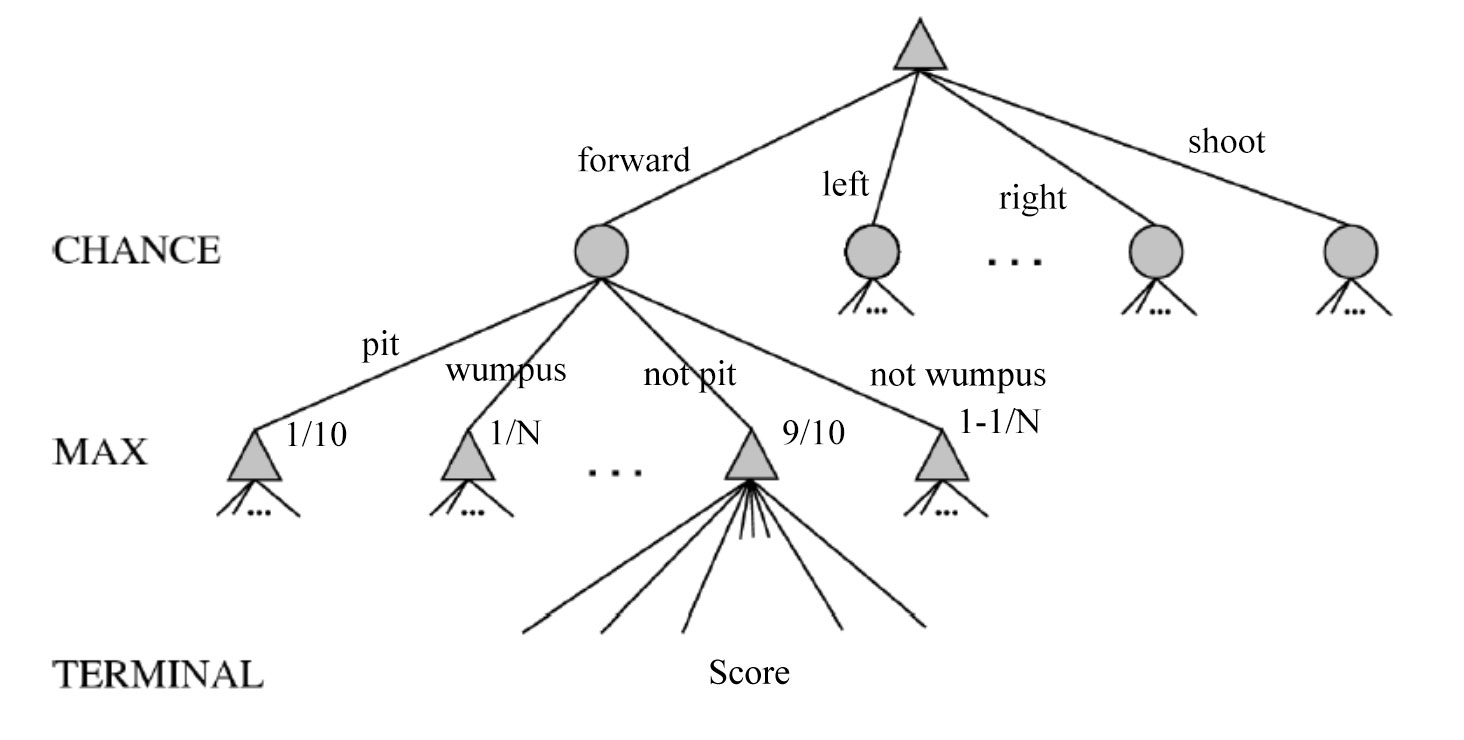
\includegraphics[width=120mm]{./pic/diagram.jpg}
    \caption{Expectimax graph}
\end{figure}

There isn't any adversary in the wumpus world and we do not know the result of an action so we used the expectimax search algorithm to maximize the score.
The expectimax algorithm use max nodes and chance nodes to determine the futur states.

We used a gameState class to keep each state of the game through the expectimax algorithm, this states include a map with the probability of a pit or the wumpus updated after each actual round.
\end{document}